\chapter{Estatística Descritiva}
\label{cap:descritiva}

Antes de escolher um teste, precisamos conhecer os dados. Quantas pessoas participaram? Há valores ausentes? As notas estão concentradas ou variam bastante? Neste capítulo, vamos usar tabelas e gráficos para responder a essas perguntas. A análise descritiva ajuda a verificar o banco e a comunicar o que foi observado; ela também orienta as análises dos próximos capítulos.

Vamos manter uma sequência simples: conferir as variáveis, descrever o centro e a dispersão e, por fim, examinar a distribuição. Os conceitos de média, mediana e moda seguem a apresentação do manual do NIST/SEMATECH e dos livros já indicados nesta apostila \parencite{NISTCentro,Triola2017}.

\section{Um conjunto de dados para praticar}

Preparei o arquivo \href{https://github.com/erickfaria/apostilaJamovi/blob/main/dados/exemplo_notas.csv}{\texttt{dados/exemplo\_notas.csv}}, disponível no repositório da apostila. Ele contém \textbf{18 pessoas fictícias}, distribuídas entre três atividades: Leitura, Vídeo e Oficina. Cada linha representa uma pessoa; as colunas \texttt{antes} e \texttt{depois} guardam duas notas dessa mesma pessoa. A coluna \texttt{horas} registra horas de estudo.

Abra o CSV no jamovi e confira os tipos: \texttt{id} como identificador, \texttt{grupo} como nominal e as demais colunas como contínuas. No arquivo, a categoria Vídeo aparece como \texttt{Video}, sem acento. Ao longo da apostila, vamos reutilizar esse banco para que você possa acompanhar o mesmo exemplo de diferentes maneiras.

\begin{tcolorbox}[colback=white,colframe=green,title={Dica de Conteúdo}]
Os dados são de elaboração própria e servem para aprender a configurar análises. Os resultados não demonstram a eficácia de uma atividade de ensino. Mantenha todos os filtros desativados, exceto quando o exercício indicar um subconjunto, e salve seu trabalho em um arquivo \texttt{.omv}.
\end{tcolorbox}

\subsection{Abrindo a análise descritiva}

No menu \textbf{Análises (Analyses)}, acesse \textbf{Exploração (Exploration)} e depois \textbf{Descritivas (Descriptives)}. Mova \texttt{depois} para \textbf{Variáveis (Variables)}. Em \textbf{Estatísticas (Statistics)}, selecione as medidas que deseja examinar. Para comparar grupos, mova \texttt{grupo} para \textbf{Dividir por (Split by)}. Essa análise oferece resumos numéricos, tabelas de frequência e gráficos \parencite{JamoviDescritivas}.

Os nomes traduzidos podem variar entre versões. Por isso, indico também os nomes em inglês. As capturas de tela dos capítulos anteriores ilustram a organização geral; registre a versão do jamovi usada no seu trabalho para facilitar a reprodução.

\section{Medidas de tendência central}

\subsection{Média}

A média aritmética é a soma dos valores dividida pelo número de observações válidas:
\[
\bar{x}=\frac{1}{n}\sum_{i=1}^{n}x_i.
\]
Para as notas $5,6,7,8,9$, a soma é $35$ e a média é $7$. Isso não significa que todas as pessoas tenham nota $7$: a média resume o conjunto em um único número.

No arquivo de exemplo, a média de \texttt{depois} é aproximadamente $64{,}56$ pontos. Ao dividir por \texttt{grupo}, você deve encontrar:

\begin{table}[H]
\centering
\caption{Resumo das notas posteriores nos dados fictícios}
\begin{tabular}{lrrr}
\hline
Atividade & $n$ & Média & Desvio padrão amostral \\
\hline
Leitura & 6 & $59{,}17$ & $7{,}03$ \\
Vídeo & 6 & $64{,}67$ & $7{,}76$ \\
Oficina & 6 & $69{,}83$ & $8{,}57$ \\
\hline
\end{tabular}
\label{tab:descritivas-notas}
\end{table}

Esses números descrevem as pessoas do arquivo. A diferença entre médias observadas, por si só, não resolve a pergunta sobre diferenças populacionais. Vamos tratar dessa distinção no capítulo de ANOVA.

\subsection{Mediana}

Para encontrar a mediana, ordenamos os valores e localizamos o centro da lista. Considere $2,12,5,10,8,7,3$. A ordenação correta é $2,3,5,7,8,10,12$; como há sete valores, o quarto é a mediana: $7$. A figura~\ref{fig:mediana-ordenada} destaca essa posição.

\begin{figure}[H]
\centering
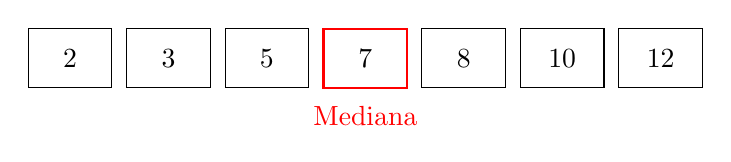
\begin{tikzpicture}[x=1.25cm,y=1cm]
  \foreach \pos/\valor in {0/2,1/3,2/5,3/7,4/8,5/10,6/12} {
    \draw (\pos,0) rectangle ++(0.85,0.75);
    \node at (\pos+0.425,0.375) {\valor};
  }
  \draw[red,thick] (3,0) rectangle (3.85,0.75);
  \node[red] at (3.425,-0.35) {Mediana};
\end{tikzpicture}
\caption{A mediana é obtida pela posição na lista ordenada. Elaboração própria.}
\label{fig:mediana-ordenada}
\end{figure}

Quando há um número par de observações numéricas, calculamos a média dos dois valores centrais. Para $2,3,5,7,8,10$, ela é $(5+7)/2=6$. A mediana pode, portanto, ser um valor que não aparece originalmente na lista.

Compare agora $5,6,7,8,9$ com $5,6,7,8,90$. A média passa de $7$ para $23{,}2$, enquanto a mediana continua igual a $7$. Esse exemplo ajuda a perceber por que convém examinar a distribuição antes de escolher um resumo. A mediana descreve a posição central; ela não equivale a dividir a área de qualquer histograma desenhado a partir da amostra exatamente ao meio.

\subsection{Moda}

A moda é o valor ou categoria com maior frequência. No conjunto $1,2,3,4,5,6,6,7,8,9,10$, o valor $6$ aparece duas vezes e cada um dos demais aparece uma vez. Assim, a moda é $6$.

\begin{figure}[H]
\centering
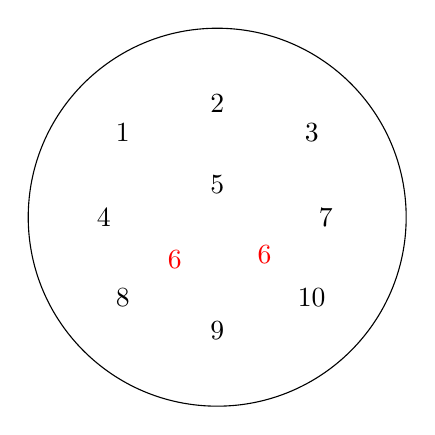
\begin{tikzpicture}[scale=1.2]
  \draw (0,0) circle (2cm);
  \foreach \px/\py/\valor in {-1/0.9/1,0/1.2/2,1/0.9/3,-1.2/0/4,0/0.35/5,1.15/0/7,-1/-0.85/8,0/-1.2/9,1/-0.85/10} {
    \node at (\px,\py) {\valor};
  }
  \node[text=red] at (-0.45,-0.45) {6};
  \node[text=red] at (0.5,-0.4) {6};
\end{tikzpicture}
\caption{O valor mais frequente está destacado em vermelho. As posições são apenas ilustrativas. Elaboração própria.}
\label{fig:circulo_moda}
\end{figure}

Pode haver empate entre valores mais frequentes. Para uma variável nominal, como meio de transporte, a moda é uma categoria; calcular a média de seus códigos não produz uma medida útil. Em variáveis contínuas, muitos valores distintos podem aparecer uma única vez. Nessa situação, observe também o histograma e não interprete uma moda isolada como um centro estável da distribuição.

\section{Medidas de dispersão}

Ter a mesma média não significa ter a mesma distribuição. Os conjuntos $4,5,6$ e $0,5,10$ têm média $5$, mas o segundo é muito mais disperso. A figura~\ref{fig:dispersao-comparacao} mostra os próprios valores, sem representar frequências como se fossem desvios padrão.

\begin{figure}[H]
\centering
\begin{tikzpicture}[x=0.85cm,y=1cm]
  \draw[->] (-0.5,0) -- (10.8,0) node[right] {Valor};
  \foreach \v in {0,2,4,5,6,8,10} {
    \draw (\v,0.07) -- (\v,-0.07) node[below] {\v};
  }
  \node[left] at (-0.5,1.5) {A};
  \node[left] at (-0.5,0.65) {B};
  \foreach \v in {4,5,6} {\fill[blue] (\v,1.5) circle (2.5pt);}
  \foreach \v in {0,5,10} {\fill[red] (\v,0.65) circle (2.5pt);}
  \draw[dashed] (5,0.2) -- (5,1.9);
  \node[above] at (5,1.9) {Média comum: 5};
\end{tikzpicture}
\caption{Mesma média, dispersões diferentes: $s_A=1$ e $s_B=5$. Elaboração própria.}
\label{fig:dispersao-comparacao}
\end{figure}

\subsection{Amplitude, variância e desvio padrão}

A amplitude total é o máximo menos o mínimo. Para $4,5,6$, vale $6-4=2$. Ela é fácil de calcular, mas depende apenas dos dois extremos.

A variância amostral e o desvio padrão amostral são dados por:
\[
s^2=\frac{\sum_{i=1}^{n}(x_i-\bar{x})^2}{n-1},
\qquad s=\sqrt{s^2}.
\]
Primeiro subtraímos a média de cada valor; depois elevamos \textbf{cada diferença} ao quadrado e somamos os quadrados. Dividimos por $n-1$ e extraímos a raiz para obter $s$. Para $4,5,6$, isso resulta em $s^2=(1+0+1)/2=1$ e $s=1$. Se somássemos as diferenças antes de elevá-las ao quadrado, obteríamos zero e perderíamos a informação sobre dispersão.

O desvio padrão volta à unidade da variável: notas em pontos têm desvio padrão em pontos, enquanto a variância fica em pontos ao quadrado. Ele não é a média aritmética das distâncias absolutas à média. A distinção entre essas medidas é apresentada pelo NIST/SEMATECH \parencite{NISTDispersao}.

Em \textbf{Descritivas}, selecione \textbf{Desvio padrão (Std. deviation)}, \textbf{Variância (Variance)} e \textbf{Amplitude (Range)}. O desvio padrão amostral de \texttt{depois}, sem divisão por grupos, é aproximadamente $8{,}60$. Não confunda essa medida com o erro padrão da média.

\subsection{Quartis e intervalo interquartil}

Os quartis resumem posições na distribuição: $Q_1$ corresponde ao percentil 25, $Q_2$ à mediana e $Q_3$ ao percentil 75. O intervalo interquartil é $IIQ=Q_3-Q_1$ e descreve a dispersão da parte central dos dados. Ao comparar cálculos manuais e softwares, confira o método de interpolação: amostras pequenas podem produzir quartis diferentes conforme a convenção usada.

O boxplot combina quartis e extremos segundo uma regra de construção. Na convenção usual de Tukey, valores além de $Q_1-1{,}5\,IIQ$ ou de $Q_3+1{,}5\,IIQ$ são sinalizados como potenciais valores atípicos. Os bigodes vão até as observações extremas que permanecem dentro desses limites \parencite{NISTBoxplot}. Um ponto sinalizado merece investigação; isso não autoriza apagá-lo automaticamente.

\subsection{Desvio padrão e erro padrão da média}

O desvio padrão descreve a variabilidade entre observações. Já o erro padrão quantifica a variabilidade amostral de um estimador. Para a média de observações independentes, estimamos:
\[
EP(\bar{x})=\frac{s}{\sqrt{n}}.
\]
No nosso exemplo, $8{,}597/\sqrt{18}\approx2{,}026$. Se você informar apenas o erro padrão, o leitor não terá uma descrição direta da dispersão das notas. Em um relatório descritivo, identifique explicitamente se os números apresentados são DP ou EP.

\section{Escolhendo tabelas e gráficos}

\subsection{Histogramas e boxplots}

Em \textbf{Gráficos (Plots)}, selecione um histograma para \texttt{depois} e compare-o com um boxplot, usando \texttt{grupo} em \textbf{Dividir por}. O histograma agrupa observações em intervalos; sua aparência depende da largura desses intervalos. O boxplot resume posições e facilita a comparação entre grupos, mas não mostra todos os detalhes da distribuição. Com apenas seis pessoas por grupo, os pontos individuais são especialmente informativos.

Procure valores incompatíveis com a escala, assimetrias e diferenças de dispersão. Uma nota $650$ em uma prova de $0$ a $100$ sugere conferir o registro original. Uma nota $100$ nessa mesma prova pode ser perfeitamente válida. Corrigir um erro documentado e excluir uma observação válida são decisões diferentes.

\subsection{Frequências para variáveis categóricas}

Para \texttt{grupo}, solicite a tabela de frequências e um gráfico de barras. Cada atividade aparece seis vezes, correspondendo a $6/18\times100\approx33{,}3\%$ das pessoas. A documentação do jamovi distingue os gráficos e as tabelas disponíveis conforme o tipo de medida \parencite{JamoviDescritivas}.

Identifique sempre o denominador de uma porcentagem. Se duas das 18 pessoas não responderam a uma pergunta, um percentual entre as 16 respostas válidas difere do percentual em relação às 18 pessoas incluídas no banco. Informe os ausentes e o número efetivamente analisado.

\section{Como relatar a análise descritiva}

Um relato possível para os dados fictícios é: ``Foram analisadas 18 observações, sem valores ausentes nas notas posteriores. A média foi de $64{,}56$ pontos, com desvio padrão amostral de $8{,}60$. As médias por atividade foram $59{,}17$, $64{,}67$ e $69{,}83$ pontos, respectivamente para Leitura, Vídeo e Oficina.''

Esse relato informa a variável, a unidade, a quantidade de observações e o significado da medida de dispersão. Acrescente um gráfico quando ele ajudar o leitor a compreender a distribuição. Antes de avançar, pratique: substitua uma nota por um valor extremo em uma cópia do arquivo, observe a mudança na média e na mediana e restaure o valor original. Guarde a versão usada em cada análise.
